%%%%%%%%%%%%%%%%%%%%%%%%%%%%%%%%%%%%%%%%%%%%%%%%%%%%%%%%%%%%%%%%%%%%%%%%%%%%%%%%
%2345678901234567890123456789012345678901234567890123456789012345678901234567890
%        1         2         3         4         5         6         7         8

\documentclass[letterpaper, 10 pt, conference]{ieeeconf}  % Comment this line out
%\usepackage{etoolbox}
%\makeatletter
%\patchcmd{\@makecaption}
%  {\scshape}
%  {}
%  {}
%  {}
%\makeatother

                                                          % if you need a4paper
%\documentclass[a4paper, 10pt, conference]{ieeeconf}      % Use this line for a4
                                                          % paper

\IEEEoverridecommandlockouts                              % This command is only
                                                          % needed if you want to
                                                          % use the \thanks command
\overrideIEEEmargins
% See the \addtolength command later in the file to balance the column lengths
% on the last page of the document



% The following packages can be found on http:\\www.ctan.org
%\usepackage{graphics} % for pdf, bitmapped graphics files
%\usepackage{epsfig} % for postscript graphics files
%\usepackage{mathptmx} % assumes new font selection scheme installed
%\usepackage{times} % assumes new font selection scheme installed
%\usepackage{amsmath} % assumes amsmath package installed
%\usepackage{amssymb}  % assumes amsmath package installed

\title{\LARGE \bf
Cross-Section Performance Reversion
}

%\author{ \parbox{3 in}{\centering Huibert Kwakernaak*
%         \thanks{*Use the $\backslash$thanks command to put information here}\\
%         Faculty of Electrical Engineering, Mathematics and Computer Science\\
%         University of Twente\\
%         7500 AE Enschede, The Netherlands\\
%         {\tt\small h.kwakernaak@autsubmit.com}}
%         \hspace*{ 0.5 in}
%         \parbox{3 in}{ \centering Pradeep Misra**
%         \thanks{**The footnote marks may be inserted manually}\\
%        Department of Electrical Engineering \\
%         Wright State University\\
%         Dayton, OH 45435, USA\\
%         {\tt\small pmisra@cs.wright.edu}}
%}

\author{Maxime Rivet, Marc Thibault and Ma{\"e}l Tr{\'e}an\\ \small Stanford University, ICME\\\tt\small mrivet, marcthib, mtrean at stanford.edu% <-this % stops a space
}
\pagestyle{plain}
\pagenumbering{arabic}

\usepackage{amsmath}
\usepackage{graphics}
\usepackage{graphicx}
\usepackage{afterpage}
\usepackage{float}  
\begin{document}
\maketitle
\thispagestyle{plain}
\pagestyle{plain}
\pagenumbering{arabic}


\begin{abstract}
This article presents a way to use cross-section correlation of returns among US equity to design a “return-to-normal” mid-frequency trading signal, the Cross-Section Performance Reversion. 

Including risk factors can significantly improve "return-to-normal" trading strategies, namely simple Mean Reversion and the Cross-Section Performance Reversion. It also ensures signal stability and better Sharpe ratios. 

This strategy exhibits a strong value potential. Even if the economic rationale behind the two strategies is comparable, the two signals are perfectly uncorrelated, which is of particular interest in a context where the Mean-Reversion is widely used in the industry. 

This cross-section strategy displays a strong sensibility to the condition numbers of the correlation matrices handled. A framework is provided to avoid numerical instabilities in these cases.

\end{abstract}
\thispagestyle{empty}
\pagestyle{empty}


%%%%%%%%%%%%%%%%%%%%%%%%%%%%%%%%%%%%%%%%%%%%%%%%%%%%%%%%%%%%%%%%%%%%%%%%%%%%%%%%


%%%%%%%%%%%%%%%%%%%%%%%%%%%%%%%%%%%%%%%%%%%%%%%%%%%%%%%%%%%%%%%%%%%%%%%%%%%%%%%%
\section{INTRODUCTION}

Mean-reversion is a widely used trading strategy in many various ways. The main idea behind it is a bet on a "return to normal" behaviour of the stocks. The normal behaviour can be the long-term price average, but can also come from a more elaborate model.

Taking advantage of the cross-correlation between stocks to design the "normal" behaviour of a stock is a natural improvement of the classical Mean-Reversion. Modeling an accurate covariance matrix is a challenging problem, as it is known that the plain historical covariance is instable and inaccurate.

This article models the covariance between stocks using a Constant-Conditional-Correlation-GARCH inspired of \cite{c1}. This model is an interesting trade off between accuracy and computational speed.

The above model allows us to have a prediction of the returns of a stock, conditioned on the market's performance. The signal is built taking into account both the predicted returns and the recent deviation of a stock from the prediction. This enables a return-to-normal signal, while taking into account the fact than some stocks tend to perform better than others on average.

The portfolio is built after hedging risk factors, which are common drivers in the performance of stocks. This makes sure that the performance of the strategy relies solely on the predictive power of the signal and not only on the performance of other outside factors. It also stabilizes the signal and tends to lower the drawdowns.

Numerical instabilities and computational problems are of crucial importance in the construction of the signal, and this paper will detail methods used to reduce the signal generation time, and to improve the stability of the strategy.

\section{SIGNAL GENERATION ON CROSS-SECTIONAL STOCKS CORRELATION}
Mean reversion assumption is that substantial price moves away from their average will be followed by a reversion to them. This hypothesis can be broadened by stating that a divergence from a model will be followed by a return to the normal modeled behavior. Stock returns here are modeled by a GARCH model and the cross-section signal is based on their residuals. 

\begin{figure}[t]
\centering
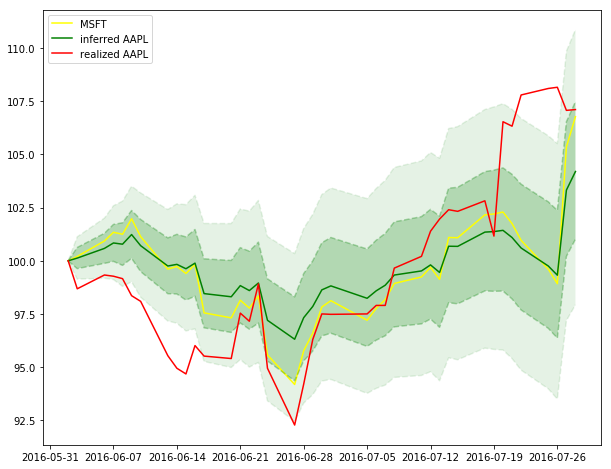
\includegraphics[width=200px]{img/diffusion.png}
\caption{Evolution of the cumulative performances of the AAPL (red) and MSFT (yellow) tickers over two months; evolution of the performance of AAPL conditional on MSFT (green) with 38\%- and 68\%-confidence intervals. The hypothesis is that the performance of AAPL (red) reverts to its ``inferred'' performance (green).}
\label{figurelabel}
\end{figure}

\subsection{Stock returns model: correlated GARCH}

The first step of the analysis is to design a single-stock time series model. This model will be individually fitted on the past time series of each stock. The goal is to provide a baseline model to each stock, in order to have a way of expressing daily "innovations" as divergences to a model. 

A useful quantity to be modeled for each stock is its log-return series. If the price of a stock at time $t$ is $P_t$, then the log-returns are defined by 

$$
r_t = \log\frac{P_{t+1}}{P_{t}}.
$$

Each series of individual log-returns is modeled with a $GARCH(1, 1)$ model. Each series alone has a mean $\mu_i$ perturbed by a noise $\epsilon_{t, i}$. The scale of these innovations, $\sigma_t$, follows an \textit{AutoRegressive Moving Average model} (ARMA) model. The main contribution here is to incorporate a correlation matrix between the normalized innovations, $R$, in order to take the market structure into account.

$$
\begin{aligned}
\textmd{returns: } \ \ &r_{t, i} = \mu_i + \epsilon_{t, i}\\
\textmd{innovations: } \ \  &\epsilon_{t} \sim \sigma_{t}.N(0, R)\\
\textmd{volatilities: }\ \ &\sigma_{t, i}^2 = w_i + \alpha_i \epsilon_{t-1, i}^2 + \beta_i \sigma_{t-1, i}^2
\end{aligned}
$$

The individual GARCH models are fitted using 200 days of past data. Once this is done, the unscaled innovations $\epsilon_{t, i}$ are extracted. The matrix $R$ is then extracted as the correlation matrix between these quantities. This fitting procedure of the coefficients of GARCH regressions and the $R$ matrix is repeated on a monthly basis. The procedure gives access, everyday, to an estimate of $\epsilon_{t}$ and $\sigma_{t}$, and a prediction of $\sigma_{t+1}$.

\subsection{Trading signal: Cross-Section Performance Reversion}

The goal of the predictive signal presented here is to incorporate the performance of a stock compared to the market environment it lies in. The first step of such an analysis is to design a model to quantify this relative performance. 

The correlated GARCH model developed previously enables closed and intuitive formulas for the conditional distribution of the returns of one stock knowing the others, as the conditioning of a normal vector. The conditional return of stock $i$, knowing the returns of other stocks $J = \{1, ...,n \} \backslash \{i\}$ can be expressed as

$$
r_{t, i}|r_{t, J} \sim N(\bar\mu, \bar\sigma^2)
$$
$$
\text{where } \left\{
                \begin{array}{ll}
               \bar\mu = \mu_{i} + \sigma_{t, i} R_{i, J} .R_{J}^{-1} .\frac{(r_{t, J} - \mu_{J})}{\sigma_{t, J}}
               \\
               \bar\sigma^2 = \sigma_{t, i}^2\big(1 - R_{i, J}.R_{J, J}^{-1}.R_{i, J}^T\big)
                \end{array}
\right..
$$

In the previous formula, subscripting vectors and matrices by $i$ corresponds to extracting the $i$-th term; while subscripting by $J$ corresponds to extracting all but the $i$-th term. The conditional mean and variance of the $i$-th stock return can be expressed given the performance of other stocks, $r_{t, J}$, and sub-matrices of the correlation matrix $R$. It can be computed at each time step, even though operations such as the inversion of $R_{J,J}$ can be computationally time-consuming. This aspect is explored in Section \ref{efficiency}.

\

This model provides with a "baseline", a model believed to be representative of the true value of a stock, and it is computed everyday for each stock, taking into account the performance of every other stock. The ensuing trading strategy is to aim at a portfolio which bets on a subsequent return to this "baseline". The price being expected based on this model gives an expected return at time $t+1$. This expected return will be the trading signal of the strategy

$$\alpha_{i, t} = \bar\mu + (\bar\mu - r_{t, i})$$

\begin{figure}[t]
\centering
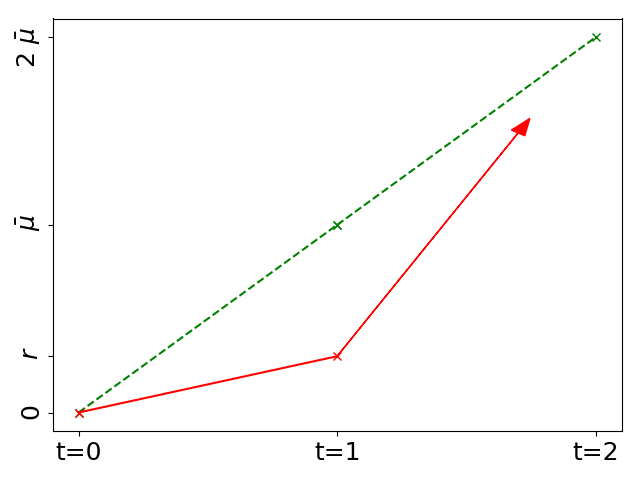
\includegraphics[width=200px]{img/explanation}
\caption{Depiction of the model's returns, realized returns, and subsequent signal. In green, cumulative returns of the studied stock under its baseline model, with daily return $\bar\mu$. In red, cumulative returns of the stock, being $r$ on the first day. In order for it to revert to the baseline, the next day's return is expected to be $2 \bar\mu - r$.}
\label{explanation}
\end{figure}

and can be decomposed in two terms: $\bar\mu$ is the baseline performance of the stock under the model as predicted above, while $\bar\mu - r_{t, i}$ is the term of reversion to the model. This formula is equivalent to a reversion-to-model in price space. 

This means that if the stock under-performed compared to the model, the portfolio's position will be long the stock; while if the stock over-performed, comparatively to the model, then the portfolio will have to be short the stock. The value of the position is given by the algebraic difference between the stock's actual performance and its performance in the model. Figure \ref{explanation} gives a graphical explanation of the interaction between the baseline model and the realized performance.

\

A clear parallel appears between the trading signal developed here and a simple mean-reversion trading strategy. Both are based on a model fitted on past data (in the case of mean reversion, the rolling mean of the stock's price; in this case the performance of the stock conditional to the other stocks' recent performance). Both produce portfolios which represent the belief that the market will revert back to the model, that is a return to the normal or expected behavior.

\subsection{Netting the market}
\label{net_market}

The primary driver to most stocks' performance can be explained solely by the overall market's performance. Consequently, the correlation between raw stock returns will mainly capture the relationship between their systematic parts. 

\begin{figure}[thpb]
\centering
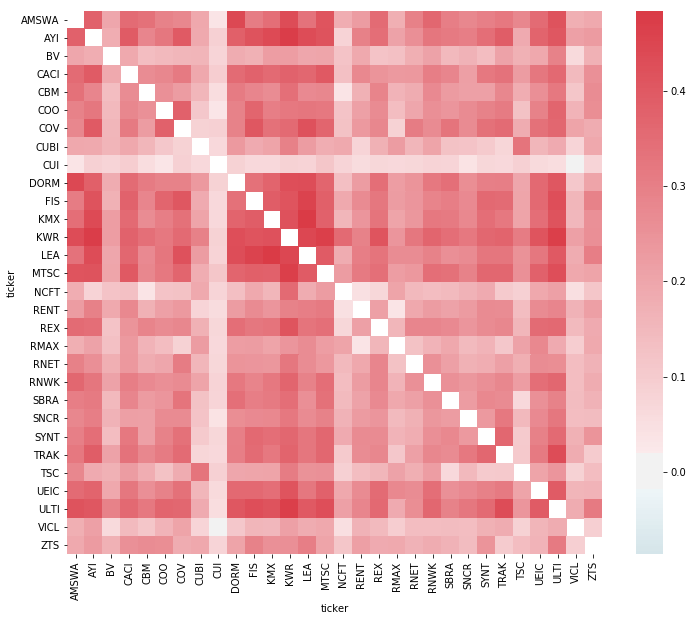
\includegraphics[width=140px]{img/bad_correlation.png}
\caption{Correlation matrix of raw returns}
\label{badcorrelation}
\end{figure}
   

Figure \ref{badcorrelation} shows the correlation matrix of the daily returns of a sample of stocks. One can see that they for the most part fluctuate around $0.3$, which is the average correlation of a stock to the others ($0.245$). This observation means that the information contained in this matrix is, in substance, the impact of the market on other stocks. Therefore, it gives little clue on the underlying correlation structure of the stocks. However, the interest here to build our signal lies in the non-systematic part of our returns.  

In order to capture the signal in the returns that is independent of the market, the decomposition is assumed to be

$$r_i(t) = \beta_i \cdot R_M(t) + \epsilon_i(t)$$ 

where $R_M$ are market returns, $r_i$ are returns of stock $i$ and $\beta_i$ is the sensitivity to the market of this stock. SPY is used as a proxy to the US market price, so that $R_M(t)$ are the SPY's daily returns. The value of interest here are the residuals, $\epsilon_i$ which are used to compute a new correlation matrix $R$. This part is crucial to build the signal described above, as it highly relies on the validity matrix. In section \ref{sectionresults} below are presented results with and without removing the systematic part of returns. Figure \ref{goodcorrelation} shows the new correlation matrix, which presents an average correlation of $0.053$. The information looks more balanced, and the stocks exhibit different relationships: correlations, decorrelations, and anticorrelations.

\begin{figure}[thpb]
\centering
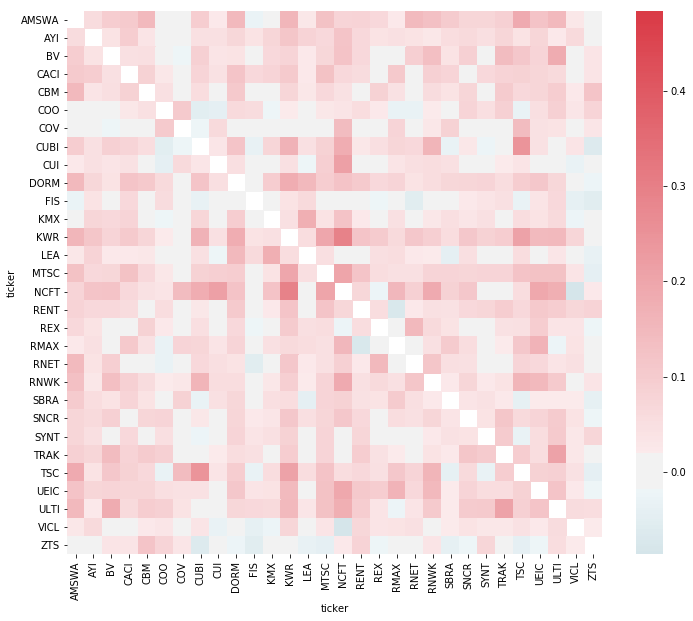
\includegraphics[width=140px]{img/good_correlation.png}
\caption{Correlation matrix of residuals returns}
\label{goodcorrelation}
\end{figure}

\section{INTEGRATION OF FACTOR RISKS AND BETA-RESIDUALS}

To construct the portfolio based on the computed signal, several risk factors have to been taken into account. Ideally, one wants its position on the market to be null on those factors. After having built them, sensitivities from each stock to these factors have to be computed.

\subsection{Computing sensitivities to factors}

Finding an equivalent of SPY for the market as proxy for other factors allows to follow the same method as for the market residuals to compute the sensitivities. As an example, the volatility factor captures the difference of performance between highly volatile stocks and low volatility stocks. One can build it by computing historical volatility, going long the first decile and short the last one. These methods gives historical ``returns'' $F^j(t)$ of each factor $j$.

After computing all the factors representing the risks to be managed in the portfolio construction process, a multivariate linear regression is performed to obtain each stock's daily sensitivity to factors. This regression is fitted daily, in a rolling manner, including a year of past data. Returns can thus be described as: $$r_i(t) = \sum_j \beta^j_i \cdot F^j(t) + \epsilon_i(t)$$

\subsection{Hedging portfolios to the considered factors}

The goal of portfolio construction is to build a market position $(w_i)$ which is as close as possible to a given input signal $(\alpha_i)$, while meeting a set of constraints. 

A basic constraint is to have a flat position, that is having a long position equal to the short position. It can be expressed by imposing $\sum_i w_i = 0$. An extra constraint is to have a null market exposure, that is making sure that the sum of the positions' sensitivities to the market is zero: $\sum_i w_i.\beta^M_i = 0$. This procedure actually stands for any risk factor, so that the considered constraint is $\sum_i w_i.\beta_i^j$ for any risk factor $j$.

In order for the hedging constraints to be met, and in order to keep a position that is consistent with the signal, the procedure that will be used here is projecting the signal $\alpha$ on the linear space orthogonal to the risk factors sensitivity vectors $\beta^j$. This operation can be performed easily by performing a simple linear regression and extracting its residuals.

\subsection{Impact of risk hedging on returns}

Basic mean reverting strategies have generally low and steady returns with some big drawdowns along the way. Risk managing the portfolio allows to cut the tails and reduce the variance of returns. 


\begin{figure}[thpb]
\centering
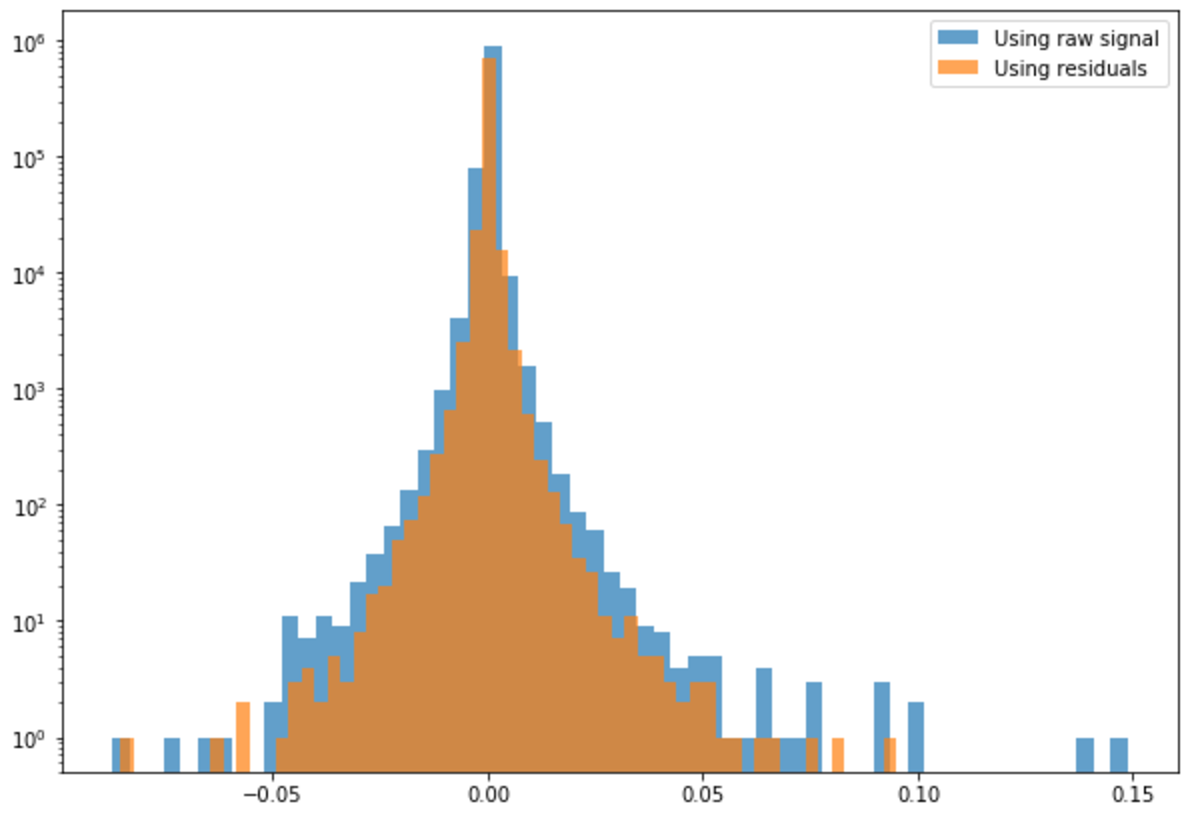
\includegraphics[width=140px]{img/diff_histo_returns.png}
\caption{Distribution of the strategy's returns without (blue) and with (orange) risk management, on a logarithmic scale. Risk hedging produces returns with much lighter tails.}
\label{histodiff}
\end{figure}

Figure \ref{histodiff} shows that the strategy returns tend to gather around the mean when risk factors are taking into account, and cut the tails. Hence, returns are more stable and the strategy has a higher Sharpe ratio. This analysis is performed in Section \ref{hedging_results}.


\section{ALGORITHM IMPLEMENTATION}

The implementation of the preceding algorithm raised several numerical problems. The bad conditioning of the correlation matrices, the extensive number of matrix inversions to be performed, and the instability of the GARCH fit were the three main concerns in the creation of the above signal.

\subsection{Numerical instability}

The raw correlation matrix of stocks returns happened to be badly conditioned, for several reasons. First, some stocks were listed with different tickers, and had very similar behaviors, leading to an almost non-invertible matrix. Secondly, when the market is not removed, the stocks are highly driven by a common component, leading to similar performances, and thus a badly conditioned matrix. The conditioned number obtained on the correlation of the most liquid 200 stocks is $\kappa = 3.78\ 10^3$.

In order to cope with this instability, two methods have been used. First, using a relaxed version of the Moore-Penrose pseudo-inverse in the estimation of the conditional mean of the stocks reduced the instability. This pseudo-inverse drops the smallest eigenvalues, thus forcing the condition number to be smaller than a target value. This operation does not lose information because the smallest eigenvalues of the correlation matrix primarily encode redundant stocks. Secondly, removing the market before generating the signal was of great use, as it reduced the impact of the common driver, made the stocks less similar, and thus increased the condition number of the correlation matrix. These two techniques enabled the reducing of the condition number of the used matrix to $\kappa = 8.30\ 10^1$.

\subsection{Computation efficiency}
\label{efficiency}

At each estimation step, the algorithm needs to invert $n_{stocks}$ sub-matrices of the correlation matrix $R$. These sub-matrices are defined by removing row $i$ and column $i$ from $R$, for every stock $i \in [n_{stocks}]$. All of those inversions are computationally heavy, as the number of stocks can get very high. Moreover, those inversions are very similar one to the other, since the $n_{stocks}$ matrices to invert are sub-matrices from the same one.

The approach taken here to ensure computational efficiency and to avoid redundant computations is using the Woodbury matrix identity. By carefully choosing matrices U ($n\times 2$) and V ($2\times n$), one can easily view the mentioned sub-matrices as rank-two perturbation of the full matrix, removing all elements but the diagonal, in a column and the corresponding row

$$
\left( 
\begin{array}{ll}
1 &0 \dots 0  \\
0 &  \\
\vdots &R_{J, J}\\
0 
\end{array}
\right) = R + U.V
$$

The Woodbury identity states that $(R + U.V)^{-1} = R^{-1} - R^{-1}U(I + VR^{-1}U)^{-1}VR^{-1}$, so that computing the inverse of $R_{J, J}$ only requires a few matrix products and a rank-two matrix inversion, with as an overhead the one-time inversion of matrix $R$. 

This implementation speeds up the time of this operation by a factor 18.3, when working with $n_{stocks}=500$, which greatly reduces the bottleneck of the algorithm. The impact of this method is further explored in Appendix \ref{inversion_section}.

\subsection{Stabilization of the GARCH}

The GARCH fitting procedure can produce very different results, as the values of $\alpha$ and $\beta$ are linked, and have to a certain extent the same role in the dynamics of the process. Thus, the value of the last volatility $\sigma_t$ is unstable, and leads to very different estimation from one day to the next.

In order to fight this problem, the GARCH fit is not performed every day, but monthly, leading to stable values of $\alpha$ and $\beta$. Moreover, the last variance of each stock is updated at each time step using the autoregression formula. This leads to a better computation time, and reduces the changes between consecutive days. These techniques of stabilization of the computation of the volatility enabled more reliable and steady signals.

\subsection{Data instability}

Another source of instability is the quality of the data. Lots of stocks present large jumps, holes and bugs. This leads to bad estimations for the GARCH, and for the correlations.

In order to solve this problem, a stock with jumps, holes or bugs in the last past $n = 100$ days is not allowed to pass the filter, and thus cannot affect the correct fits. When a new stock passed the filter, the GARCH is evaluated only on this stock, and the correlation with this stock is computed. When a stock disappears, it is only removed from the correlation matrix.

\section{RESULTS}
\label{sectionresults}
\subsection{Universe}

The universe that is being considered is the 100 most traded stocks in the United States. This offers good guaranties of liquidity and data availability.

\subsection{Baseline}

The baseline that will be built upon and compared to is the basic framework of the Cross-Section Performance Reversion, using the correlation matrix of raw returns, and without hedging the portfolio.

As expected in Section \ref{net_market}, the signal is not strong and has very low performance, with a Sharpe ratio of $0.263$. Figure \ref{bad_result} shows the behavior of the unhedged portfolio with this signal. This shows that correctly estimating the correlation matrix is central in the signal construction.



\begin{figure}[thpb]
\centering
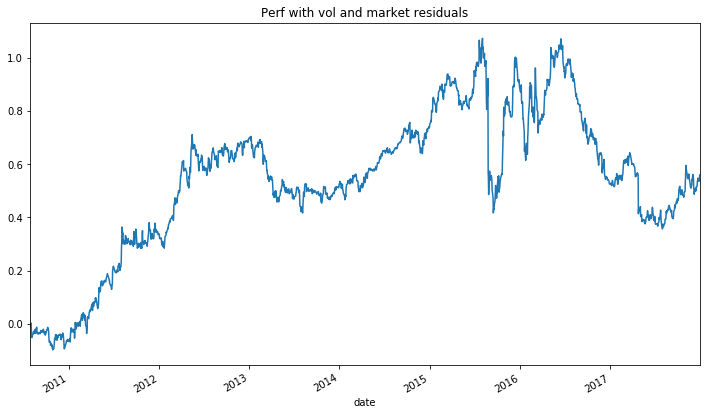
\includegraphics[width=140px]{img/Fit_vanilla_execute_vanilla.png}
\caption{Portfolio performance with baseline signal, trading daily between 2011 and 2017. Returns are highly unstable, and can be interpreted as noise. Sharpe = $0.263$.}
\label{bad_result}
\end{figure}

\subsection{Netting the market on the signal}

Netting out the market before generating the signal improved significantly the performance of the strategy. It led to more relevant estimations of the true correlations between stocks. Moreover, it significantly improves the conditioning of the correlation matrix, since the stocks' returns have been made independent from a common driving factor, the market.

The results are significantly better, as figure \ref{fit_residuals} shows. The Sharpe ratio is $0.972$.

\begin{figure}[thpb]
\centering
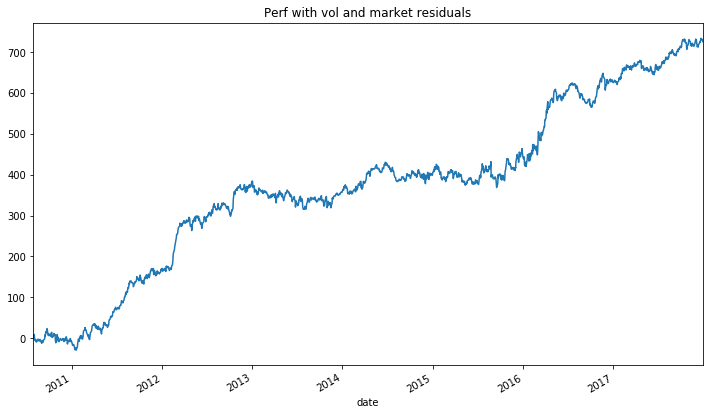
\includegraphics[width=140px]{img/Fit_residuals_markt_argsort_execute_mkt_vol.png}
\caption{Portfolio performance with market fit signal. Returns are steadier are more reliably positive. Sharpe = $0.972$.}
\label{fit_residuals}
\end{figure}

Another signal can be extracted from the above method: the stocks can be ranked according to the value of the signal computed as above, and this rank becomes the signal on which to trade. This methods helps removing outliers, and is a safety test of the robustness of the signal. This new signal performs comparably to the original one, with a Sharpe ratio of $0.914$.

\subsection{Hedging risk factors in the portfolio construction}
\label{hedging_results}

Hedging risk is the final step in the portfolio construction. It helps removing the common drivers in the market, and trade the real alpha present in the signal. This provides a large improvement in the performance of the strategy. Table \ref{Sharpe} demonstrates the impact of hedging the market and the volatility. The Sharpe ratio reaches $1.278$ after the hedge. Figure \ref{best_performance} shows the performance of this portfolio with the ranked signal presented above.

\begin{figure}[thpb]
\centering
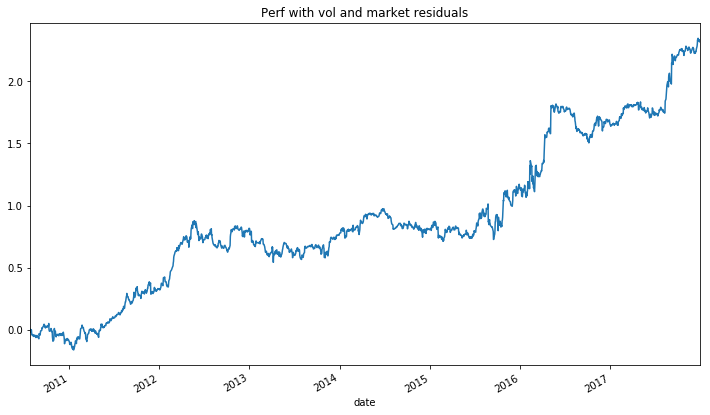
\includegraphics[width=140px]{img/Fit_residuals_mkt_execute_vanilla.png}
\caption{Portfolio performance with market fit signal, hedging market and volatility. Returns have better performance. Sharpe = $1.278$.}
\label{best_performance}
\end{figure}

Overall, the holding period is close to $2.85$ days, as Table \ref{Holding} shows. However, this value is to be taken with care, as there are numerous holes in the data that make the holding period computation inaccurate. The actual holding period is expected to be longer than this. 

\subsection{Comparison with standard mean-reversion}

This signal is totally uncorrelated with the standard mean-reversion strategy. This feature makes it very appealing, as it makes it less likely to suffer overuse and market saturation as a widely adopted mean reversion strategy could experience. Moreover, there is still work to be done to improve the performance and the stability of the strategy.  

\section{PROSPECTIVE ENHANCEMENTS}

\subsection{Universe}
In order to test the strength of the signal more thoroughly, the same study could be conducted on other universes. The number of stocks was maintained low to avoid aforementioned stability issues, and a natural extension of this work would be to extend the number of stocks traded.

\subsection{Signal construction}

Due to the numerical instabilities and to noise in the dataset, the signal can lead to a very high exposition to certain stocks. Computing a modified signal with ranks instead of raw signal helps reducing this problem, but further numerical studies could reduce those instabilities. 

\subsection{Risk management}

The portfolio is only built hedging two main risk factors, which are market and volatility. Several important risk factors have not been dealt with here: momentum, value, quality... Hedging industry sectors would also be of great interest for the stability of the portfolio. Also, constructing the signal by sector could also be a solution to avoid numerical instabilities stemming from the estimation of large correlation matrices. 

\section{CONCLUSION}

This paper deals presents a innovation to the standard, widely used mean-reversion strategy. Incorporating cross-correlations in the estimation of the signal, this method captures an additional source of information in the construction of the signal.

Hedging properly risk factors is crucial in the construction of the portfolio, as it stabilizes the signal, and makes sure that the signal is not taking bets on the market or any risk factor.

The results are promising, as this signal is totally uncorrelated to the standard mean-reversion. More work would be needed to stabilize the signal, to explore the hyperparameters space and to hedge more risk factors.

%\addtolength{\textheight}{-12cm}   % This command serves to balance the column lengths
                                  % on the last page of the document manually. It shortens
                                  % the textheight of the last page by a suitable amount.
                                  % This command does not take effect until the next page
                                  % so it should come on the page before the last. Make
                                  % sure that you do not shorten the textheight too much.

%%%%%%%%%%%%%%%%%%%%%%%%%%%%%%%%%%%%%%%%%%%%%%%%%%%%%%%%%%%%%%%%%%%%%%%%%%%%%%%%



%%%%%%%%%%%%%%%%%%%%%%%%%%%%%%%%%%%%%%%%%%%%%%%%%%%%%%%%%%%%%%%%%%%%%%%%%%%%%%%%





\section*{ACKNOWLEDGMENT}

We thank Lisa Borland for her high-quality teaching, and for gathering such interesting speakers, during the MS\&E448 class. Her supervision and her technical insights were crucial to the success of this study. We also thank Enguerrand Horel for organizing the class. 



%%%%%%%%%%%%%%%%%%%%%%%%%%%%%%%%%%%%%%%%%%%%%%%%%%%%%%%%%%%%%%%%%%%%%%%%%%

\begin{thebibliography}{99}

\bibitem{c1} Bollerslev, Tim (1990). Modelling the coherence in short-run nominal exchange rates: A multivariate generalized ARCH model, Review of Economics and Statistics, 72, 498-505. 






\end{thebibliography}

\pagebreak

\begin{appendices}
\onecolumn

\section{Matrix inversion optimization}
\label{inversion_section}

\begin{table}[!h]
\centering
\caption{Comparison of the performance for sub-matrix inversion methods}
\label{inversion_table}
\begin{tabular}{|r|c|c|c|}\hline
Matrix size & Woodbury inversions & Classical inversions & Speedup \\ \hline
$n = 10$ & $8.02\ 10^{-4}$ & $1.46\ 10^{-3}$ & 1.82 \\ \hline
$n = 50$ & $6.08\ 10^{-3}$ & $4.30\ 10^{-2}$ & 7.06 \\ \hline
$n = 100$ & $3.51\ 10^{-2}$ & $4.48\ 10^{-1}$ & 12.7 \\ \hline
$n = 200$ & $1.61\ 10^{-1}$ & $2.57\ 10^{0}$ & 16.0 \\ \hline
$n = 500$ & $2.70\ 10^{0}$ & $4.94\ 10^{1}$ & \textbf{18.3} \\ \hline
\end{tabular}
\end{table}

One computational bottleneck of the developed algorithm is the inversion of the $n_{stocks}$ sub-matrices of the correlation matrix $R$. The method developed in section \ref{efficiency}, relying on fast inversion of the sub-matrices by considering them as rank-two perturbations of the main matrix $R$, yields a significant performance increase. This method will be described as ``Woodbury inversions'', compared to the ``Classical inversions'' method, which extracts and inverts sequentially the $n_{stocks}$ sub-matrices. The benchmark was conducted using the correlation matrices of random $n_{stocks} \times 6\ n_{stocks}$ matrices, and its results are reported in seconds. As described in Table \ref{inversion_table}, this method is especially efficient when working with a large array of stocks. 

\section{Performance and result tables}

The following tables shows the results of the three different signals. The first signal is obtained through the correlation matrix of the raw returns. The second signal is obtained with the correlation of the returns net of the market. The third signal is obtained from the second by ranking the values and using the rank as the signal. Hedging the risk factors highly increases the performance. The ranked signal has a Sharpe ratio comparable to the normal signal, but has a much lower variance, as seen in the return per trade table.

\begin{table}[H]
\caption{Sharpe ratios}
\label{Sharpe}
\centering
\begin{tabular}{|r|c|c|c|}\hline
Hedge $\backslash$ Signal & Raw returns & Market net returns & Mkt net + ranked \\ \hline
No hedge & 0.263 & 0.972 & 0.914 \\
Hedge market & 0.517 & 1.067 & 1.019 \\
Hedge vol & 0.410 & 1.158 & 1.203 \\
Hedge mkt and vol & 0.520 & 1.235 & \textbf{1.278} \\ \hline
\end{tabular}
\end{table}

\begin{table}[H]
\centering
\caption{Return per trade (\%)}
\begin{tabular}{|r|c|c|c|}\hline
Hedge $\backslash$ Signal & Raw returns & Market net returns & Mkt net + ranked \\ \hline
No hedge & 0.010 & 0.028 & 0.018 \\
Hedge market & 0.019 & 0.031 & 0.021 \\
Hedge vol & 0.014 & 0.032 & 0.022 \\
Hedge mkt and vol & 0.018 & \textbf{0.034} & 0.023 \\ \hline
\end{tabular}
\end{table}

\begin{table}[H]
\centering
\caption{Holding period}
\label{Holding}
\begin{tabular}{|r|c|c|c|}\hline
Signal & Raw returns & Market net returns & Mkt net + ranked \\ \hline
Holding period & 2.84 & 2.86 & 2.86 \\ \hline
\end{tabular}
\end{table}

\end{appendices}


\end{document}
